% SIAM Supplemental File Template
\documentclass[review,supplement,onefignum,onetabnum]{siamonline220329}

% SIAM Shared Information Template
\documentclass[preprint,onefignum,onetabnum]{siamart220329}

% This is information that is shared between the main document and any
% supplement. If no supplement is required, then this information can
% be included directly in the main document.


% Packages and macros go here
\usepackage{lipsum}
\usepackage{amssymb}
\usepackage{amsfonts}
\usepackage{graphicx}
\usepackage{epstopdf}
\usepackage{algorithmic}
\usepackage{tikz}
\usepackage{pgfplots}
\usetikzlibrary{shapes.arrows, patterns, calc}
\usepackage{tikz-3dplot}
\usepackage{bbm}
\usepackage{bm}
\ifpdf
  \DeclareGraphicsExtensions{.eps,.pdf,.png,.jpg}
\else
  \DeclareGraphicsExtensions{.eps}
\fi
\usepackage{todonotes}

\definecolor{lightblue}{HTML}{a1b4c7}
\definecolor{orange}{HTML}{ea8810}
\definecolor{silver}{HTML}{b0aba8}
\definecolor{rust}{HTML}{b8420f}
\definecolor{seagreen}{HTML}{23553c}

\colorlet{lightsilver}{silver!30!white}
\colorlet{darkorange}{orange!85!black}
\colorlet{darksilver}{silver!85!black}
\colorlet{darklightblue}{lightblue!85!black}
\colorlet{darkrust}{rust!85!black}
\colorlet{darkseagreen}{seagreen!85!black}

\hypersetup{
  colorlinks=true,
  linkcolor=darkrust,
  citecolor=darkseagreen,
  urlcolor=darksilver
}

\pgfplotsset{compat=newest}
\usepgfplotslibrary{fillbetween}

% custom commands:
% \newcommand{\todo}[1]{{\color{red} #1}}
\newcommand{\Ftodo}[1]{\todo[color=lightblue]{Florian: #1}}
\newcommand{\Stodo}[1]{\todo[color=seagreen]{Stephen: #1}}

\usepackage{mathtools}
%Names of standard objects
\newcommand*{\Reals}{\mathbb{R}}
\newcommand*{\Naturals}{\mathbb{N}}

\makeatletter
\renewcommand{\paragraph}{%
  \@startsection{paragraph}{4}%
  {\z@}{1.0ex \@plus .5ex \@minus .2ex}{-.7em}%
  {\normalfont\normalsize\bfseries}%
}
\makeatother

% From https://tex.stackexchange.com/questions/198771/align-in-substack
\makeatletter
\newcommand{\subalign}[1]{%
  \vcenter{%
    \Let@ \restore@math@cr \default@tag
    \baselineskip\fontdimen10 \scriptfont\tw@
    \advance\baselineskip\fontdimen12 \scriptfont\tw@
    \lineskip\thr@@\fontdimen8 \scriptfont\thr@@
    \lineskiplimit\lineskip
    \ialign{\hfil$\m@th\scriptstyle##$&$\m@th\scriptstyle{}##$\hfil\crcr
      #1\crcr
    }%
  }%
}
\makeatother

%Names of Variables:
\newcommand*{\stateP}{\mathbf{x}}
\newcommand*{\stateD}{\hat{\mathbf{x}}}

\newcommand*{\resP}{\mathbf{r}}
\newcommand*{\resD}{\hat{\mathbf{r}}}

\newcommand*{\resMatP}{\mathbf{R}}
\newcommand*{\resMatD}{\hat{\mathbf{R}}}


\newcommand*{\dirP}{\mathbf{p}}
\newcommand*{\dirMatP}{\mathbf{P}}
\newcommand*{\dirD}{\hat{\mathbf{p}}}
\newcommand*{\dirMatD}{\hat{\mathbf{P}}}

\newcommand*{\rhsP}{\mathbf{b}}
\newcommand*{\rhsD}{\hat{\mathbf{b}}}

\newcommand*{\mat}{\mathbf{A}}
\newcommand*{\adj}[1]{#1^{\dagger}}
\newcommand*{\con}[1]{\bar{#1}}

\newcommand*{\alphaP}{\alpha}
\newcommand*{\alphaD}{\hat{\alpha}}

\newcommand*{\alphaMatP}{\bm{\alpha}}
\newcommand*{\alphaMatD}{\hat{\bm{\alpha}}}

\newcommand*{\betaP}{\beta}
\newcommand*{\betaD}{\hat{\beta}}

\newcommand*{\betaMatP}{\bm{\beta}}
\newcommand*{\betaMatD}{\hat{\bm{\beta}}}

\renewcommand{\vec}[1]{\bm{#1}}

\renewcommand{\algorithmicrequire}{\textbf{Input:}}
\renewcommand{\algorithmicensure}{\textbf{Output:}}

% Add a serial/Oxford comma by default.
\newcommand{\creflastconjunction}{, and~}

% Used for creating new theorem and remark environments
\newsiamremark{remark}{Remark}
\newsiamremark{hypothesis}{Hypothesis}
\newsiamremark{example}{Example}
\crefname{hypothesis}{Hypothesis}{Hypotheses}
\newsiamthm{claim}{Claim}

% Sets running headers as well as PDF title and authors
\headers{Factorization by greedy conditional selection}{
S. Huan, J. Guinness, M. Katzfuss, H. Owhadi, F. Sch{\"a}fer}

% Title. If the supplement option is on, then "Supplementary Material"
% is automatically inserted before the title.
\title{Sparse Cholesky factorization by greedy conditional selection}

% Authors: full names plus addresses.
\author{
  Stephen\ Huan\thanks{Georgia Institute of Technology} \and
  Joe\ Guinness\thanks{Joe} \and
  Matthias\ Katzfuss\thanks{Matthias} \and
  Houman\ Owhadi\thanks{Houman} \and
  Florian\ Sch{\"a}fer\thanks{Georgia Institute of Technology,
  S1317 CODA, 756 W Peachtree St Atlanta, GA 30332, \newline
  \email{florian.schaefer@cc.gatech.edu},\newline Corresponding Author}
}


\usepackage{amsopn}
\DeclareMathOperator{\diag}{diag}
\let\trace\relax
\DeclareMathOperator{\trace}{trace}
\DeclareMathOperator{\logdet}{logdet}
\DeclareMathOperator{\chol}{chol}

\DeclareMathOperator*{\argmin}{argmin}

\DeclareMathOperator{\E}{E}
\DeclareMathOperator{\Var}{Var}
\DeclareMathOperator{\Cov}{Cov}
\DeclareMathOperator{\Corr}{Corr}
\DeclareMathOperator{\I}{MI}
\DeclareMathOperator{\entropy}{H}

%%% Local Variables:
%%% mode:latex
%%% TeX-master: "ex_article"
%%% End:


\externaldocument{experimental_design_linalg}

% Optional PDF information
\ifpdf
\hypersetup{
  pdftitle={%
    Supplementary Materials: Sparse Cholesky
    factorization by greedy conditional selection
  },
  pdfauthor={S. Huan, J. Guinness, M. Katzfuss, H. Owhadi, F. Sch{\"a}fer}
}
\fi

\begin{document}

\maketitle

\section{Derivations in KL-minimization}

\subsection{Aggregated computation of sparsity entries}
\label{app:L_mult}

We wish to compute the entries of the sparse Cholesky factor
\( L_{s_i, i} \) according to \cref{eq:L_col} in the aggregated
sparsity setting of \cref{subsec:aggregated}.
Recall that we have aggregated the column indices \( i_1 \succ
\dotsb \succ i_m \) into \( \tilde{i} = \{ i_1, \dotsc, i_m \} \)
and \( s_{\tilde{i}} \) denotes the aggregated sparsity pattern.
The sparsity pattern for the \( i \)th column of the group is all
those entries that satisfy lower triangularity, \( s_i \defeq \{
j \in s_{\tilde{i}} : j \succeq i \} \subseteq s_{\tilde{i}} \).
Because each column's sparsity pattern is a subset of the
overall sparsity pattern, it is possible to compute an outer
approximation and specialize to each column efficiently.
Assuming the sparsity entries \( s_{\tilde{i}} \) are sorted according to
\( \prec \), let \( Q \defeq \CM_{s_{\tilde{i}}, s_{\tilde{i}}}^{-1} \) be
the precision of the aggregated sparsity pattern and let \( k \) be the \(
i \)th column's index in \( s_{\tilde{i}} \).
Because \( s_{\tilde{i}} \) is sorted according to \(
\prec \), the sparsity pattern for the \( i \)th column
\( s_i \) is exactly the entries \( k \) and after,
\begin{align}
  \label{eq:L_precision}
  L_{s_i, i}
   &= \frac{\CM_{s_i, s_i}^{-1} \vec{e}_1}
           {\sqrt{\vec{e}_1^{\top} \CM_{s_i, s_i}^{-1} \vec{e}_1}}
    = \frac{\left (Q^{-1} \right )_{k:, k:}^{-1} \vec{e}_1}
           {\sqrt{\vec{e}_1^{\top} \left (Q^{-1} \right )_{k:, k:} \vec{e}_1}}
    = \frac{Q_{k:, k: \mid :k - 1} \vec{e}_1}
           {\sqrt{\vec{e}_1^{\top} Q_{k:, k: \mid :k - 1} \vec{e}_1}}
\end{align}
where the first equality follows from \( Q^{-1} =
\CM_{s_{\tilde{i}}, s_{\tilde{i}}} \) and \( s_i \) is
the \( k \)th index of \( s_{\tilde{i}} \) and after.
We turn marginalization in precision into
conditioning in covariance by \cref{eq:inverse_cond}.

So we want the \( k \)th column of \( Q
\), conditional on all columns before it.
From \cref{eq:chol}, this can be directly read off the \(
k \)th column of the Cholesky factor \( L = \chol(Q) \) to
compute \cref{eq:L_col} for each \( i \in \tilde{i} \).
However, computing \( Q = \CM_{s_{\tilde{i}}, s_{\tilde{i}}}^{-1} \) by
inverting \( \CM_{s_{\tilde{i}}, s_{\tilde{i}}} \) and then additionally
computing its Cholesky factor \( L = \chol(Q) \) is a bit wasteful.

Instead of computing a \emph{lower} triangular factor for the precision,
we can compute an \emph{upper} triangular factor for the covariance whose
inverse transpose will be a lower triangular factor for the precision.
Let \( U = P^{\Reverse} \chol(P^{\Reverse} \CM_{s_{\tilde{i}},
s_{\tilde{i}}} P^{\Reverse}) P^{\Reverse} \) where \( P^{\Reverse} \) is the
order-reversing permutation; \( U \) is upper triangular and satisfies \( U
U^{\top} = \CM_{s_{\tilde{i}}, s_{\tilde{i}}} \) so \( U^{-\top} U^{-1} =
\CM_{s_{\tilde{i}}, s_{\tilde{i}}}^{-1} = Q \) and we see that \( L = U^{-\top}
\) is a lower triangular factor satisfying \( L L^{\top} = Q \).
Thus we can compute \( U \) as a Cholesky factor of the covariance
and dynamically form the \( k \)th column of \( L \) by solving
the triangular system \( L_{:, k} = U^{-\top} \vec{e}_k \).
This method is described in Algorithm 3.2, Figure
4, and Appendix A.2 of \cite{schafer2021sparse}.

\newpage

\section{Computation in sparse Gaussian process selection}

\subsection{Mutual information objective}
\label{app:mutual_info}

The \emph{mutual information} or \emph{information
gain} between two collections of random variables \(
\vec{y}_\Pred \) and \( \vec{y}_\Train \) is defined as
\begin{align}
  \label{eq:info}
  \MI[\vec{y}_\Pred;\vec{y}_\Train] &\defeq \entropy[\vec{y}_\Pred] -
    \entropy[\vec{y}_\Pred \mid \vec{y}_\Train].
\end{align}
Maximizing the mutual information is equivalent to minimizing the
conditional entropy since the entropy of \( \vec{y}_\Pred \) is constant.
Because the differential entropy of a multivariate Gaussian monotonically
increases with the determinant of its covariance matrix, minimizing the
conditional entropy is equivalent to minimizing the determinant of the
posterior covariance matrix.
The determinant of a single prediction point is its variance so we
can minimize the \emph{conditional variance} of the target point.

Supposing \( \vec{y}_\Pred \) is estimated by the posterior
mean \cref{eq:cond_mean}, the estimator is unbiased because \(
\E[\E[\vec{y}_\Pred \mid \vec{y}_\Train]] = \E[\vec{y}_\Pred] \) and
so the expected mean squared error of the estimator \( \text{MSE}
\defeq \E[(\vec{y}_\Pred - \E[\vec{y}_\Pred \mid \vec{y}_\Train])^2]
\) is simply the conditional variance because
\begin{align}
  \text{MSE}
  = \E[\E[(\vec{y}_\Pred - \E[\vec{y}_\Pred \mid \vec{y}_\Train])^2
          \mid \vec{y}_\Train]]
  = \E[\Var[\vec{y}_\Pred \mid \vec{y}_\Train]]
  = \Var[\vec{y}_\Pred \mid \vec{y}_\Train],
\end{align}
from the quirk that the posterior covariance \cref{eq:cond_cov}
does not depend on observing  \( \vec{y}_\Train \).

So maximizing the mutual information is equivalent to minimizing the
posterior variance (or log determinant) which is in turn equivalent
to minimizing the expected mean squared error of the prediction.
Yet another perspective arises from comparing the definition of mutual
information \cref{eq:info} to the EV-VE identity \cref{eq:eve},
\begin{align}
  \label{eq:info_eve}
  \textcolor{darkorange}{\entropy[\vec{y}_\Pred]} &=
    \textcolor{lightblue}{\entropy[\vec{y}_\Pred \mid \vec{y}_\Train]} +
         \textcolor{rust}{\MI[\vec{y}_\Pred;\vec{y}_\Train]} \\
  \label{eq:eve}
  \textcolor{darkorange}{\Var[\vec{y}_\Pred]} &=
    \textcolor{lightblue}{\E[\Var[\vec{y}_\Pred \mid \vec{y}_\Train]]} +
         \textcolor{rust}{\Var[\E[\vec{y}_\Pred \mid \vec{y}_\Train]]}
\end{align}
On the left hand side, \textcolor{darkorange}{variance}
is monotone with \textcolor{darkorange}{entropy}.
On the right-hand side, the \textcolor{lightblue}{conditional
variance} is monotone with \textcolor{lightblue}{conditional entropy}.
Because the two terms on the right-hand side add to a constant, minimizing
the \textcolor{lightblue}{conditional variance} is equivalent to maximizing
the \textcolor{rust}{variance of conditional expectation}, which, by process
of elimination, corresponds to the \textcolor{rust}{mutual information}.
We can intuitively interpret the variance of the conditional expectation
as measuring the extent to which the estimator for \( \vec{y}_\Pred \),
the conditional expectation \( \E[\vec{y}_\Pred \mid \vec{y}_\Train] \),
varies with observed values of \( \vec{y}_\Train \).

\subsection{Cholesky factorization as iterative conditioning}
\label{app:chol_stat}

Factoring the joint covariance matrix \( \CM \) blocked as
\cref{eq:inverse_cond} by two steps of block Gaussisan elimination,
\begin{align}
  \nonumber
  \begin{pmatrix}
    \CM_{1, 1} & \CM_{1, 2} \\
    \CM_{2, 1} & \CM_{2, 2}
  \end{pmatrix} &=
  \begin{pmatrix}
    \Id & 0 \\
    \textcolor{darkorange}{\CM_{2, 1} \CM_{1, 1}^{-1}} & \Id
  \end{pmatrix}
  \begin{pmatrix}
    \CM_{1, 1} & 0 \\
    0 & \textcolor{lightblue}{
      \CM_{2, 2} - \CM_{2, 1} \CM_{1, 1}^{-1} \CM_{1, 2}
    }
  \end{pmatrix}
  \begin{pmatrix}
    \Id & \textcolor{darkorange}{\CM_{1, 1}^{-1} \CM_{1, 2}} \\
    0 & \Id
  \end{pmatrix}
  \shortintertext{
    so we see that the Cholesky factorization
    of the joint covariance \( \CM \) is
  }
  \chol(\CM) &=
  \begin{pmatrix}
    \Id & 0 \\
    \textcolor{darkorange}{\CM_{2, 1} \CM_{1, 1}^{-1}} & \Id
  \end{pmatrix}
  \begin{pmatrix}
    \chol(\CM_{1, 1}) & 0 \\
    0 & \chol(\textcolor{lightblue}{
      \CM_{2, 2} - \CM_{2, 1} \CM_{1, 1}^{-1} \CM_{1, 2}
    })
  \end{pmatrix} \\
  \label{eq:chol}
  &=
  \begin{pmatrix}
    \textcolor{darkorange}{\chol(\CM_{1, 1})} & 0 \\
    \textcolor{darkorange}{\CM_{2, 1} \chol(\CM_{1, 1})^{-\top}} &
    \chol(\textcolor{lightblue}{
      \CM_{2, 2} - \CM_{2, 1} \CM_{1, 1}^{-1} \CM_{1, 2}
    })
  \end{pmatrix}
\end{align}
where the conditional expectation \cref{eq:cond_mean} corresponds
to \( \textcolor{darkorange}{\CM_{2, 1} \CM_{1, 1}^{-1}} \) and
the conditional covariance \cref{eq:cond_cov} corresponds to
\(
  \textcolor{lightblue}{\CM_{2, 2} - \CM_{2, 1} \CM_{1, 1}^{-1} \CM_{1, 2}}
\).
Blocking \( \CM \) such that 1 is the current column and 2 is
all the indices past 1, we observe the column of the Cholesky
factor is a conditional covariance \( \CM_{2, 1} \) divided by
\( \chol(\CM_{1, 1})^{\top} \), the square root of the variance
(the Cholesky factor of a scalar is its square root).
We conclude that the \( k \)th column of the Cholesky factor equals \( \vec{u}
\) in \cref{eq:cond_select} since iteratively conditioning on the columns \(
i_1, i_2, \dotsc, i_{k - 1} \) is equivalent to conditioning on \( \I \) by the
quotient rule \cref{eq:quotient_rule}.

\subsection{Updating precision after insertion}
\label{app:prec_insert}

Given the precision matrix \( \CM_{1, 1}^{-1} \) we wish to
compute the inverse of the covariance matrix \( \CM_{1, 1} \)
with added rows and columns, i.e. to compute \( \CM^{-1} \) for
\(
  \CM =
    \begin{pmatrix}
      \CM_{1, 1} & \CM_{1, 2} \\
      \CM_{2, 1} & \CM_{2, 2}
    \end{pmatrix}
\).
Using the same block \( L D L^{\top} \) factorization as \cref{eq:chol} with
the Schur complement \textcolor{lightblue}{\( \CM_{2, 2} - \CM_{2, 1} \CM_{1,
1}^{-1} \CM_{1, 2} \)} denoted \textcolor{lightblue}{\( \CM_{2, 2 \mid 1} \)},
\begin{align}
  \begin{pmatrix}
    \CM_{1, 1} & \CM_{1, 2} \\
    \CM_{2, 1} & \CM_{2, 2}
  \end{pmatrix} &=
  \begin{pmatrix}
    \Id & 0 \\
    \textcolor{darkorange}{\CM_{2, 1} \CM_{1, 1}^{-1}} & \Id
  \end{pmatrix}
  \begin{pmatrix}
    \CM_{1, 1} & 0 \\
    0 & \textcolor{lightblue}{\CM_{2, 2 \mid 1}}
  \end{pmatrix}
  \begin{pmatrix}
    \Id & \textcolor{darkorange}{\CM_{1, 1}^{-1} \CM_{1, 2}} \\
    0 & \Id
  \end{pmatrix}.
  \shortintertext{Inverting both sides of the equation and multiplying,}
  \CM^{-1} &=
  \begin{pmatrix}
    \Id & -\textcolor{darkorange}{\CM_{1, 1}^{-1} \CM_{1, 2}} \\
    0 & \Id
  \end{pmatrix}
  \begin{pmatrix}
    \CM_{1, 1}^{-1} & 0 \\
    0 & \textcolor{lightblue}{\CM_{2, 2 \mid 1}^{-1}}
  \end{pmatrix}
  \begin{pmatrix}
    \Id & 0 \\
    -\textcolor{darkorange}{\CM_{2, 1} \CM_{1, 1}^{-1}} & \Id
  \end{pmatrix} \\
  &=
  \begin{pmatrix}
    \CM_{1, 1}^{-1} +
    \textcolor{darkorange}{
      \left (\CM_{1, 1}^{-1} \CM_{1, 2} \right )
    } \textcolor{lightblue}{\CM_{2, 2 \mid 1}^{-1}}
    \textcolor{darkorange}{
      \left (\CM_{2, 1} \CM_{1, 1}^{-1} \right )
    } &
    - \textcolor{darkorange}{
      \left (\CM_{1, 1}^{-1} \CM_{1, 2} \right )
    } \textcolor{lightblue}{\CM_{2, 2 \mid 1}^{-1}} \\
    - \textcolor{lightblue}{\CM_{2, 2 \mid 1}^{-1}} \textcolor{darkorange} {
      \left (\CM_{2, 1} \CM_{1, 1}^{-1} \right )
    } & \textcolor{lightblue}{\CM_{2, 2 \mid 1}^{-1}}
  \end{pmatrix}.
  \shortintertext{
    In the context of adding a new entry \( k \) to the
    matrix, \( \CM_{1, 1} = \CM_{\I, \I} \), \( \CM_{1, 2}
    = \CM_{\I, k} \), and \( \CM_{2, 2} = \CM_{k, k} \).
    Also note that \( \textcolor{lightblue}{\CM_{k, k \mid \I}^{-1}}
    \) is the precision of \( k \) conditional on the entries in \(
    \I \), which has already been computed in \cref{alg:select_prec}.
    If we let \( \vec{v} \defeq \textcolor{darkorange}{\CM_{\I,
    \I}^{-1} \CM_{\I, k}} \), then
  }
  &=
  \begin{pmatrix}
    \CM_{\I, \I}^{-1} + \CM_{k, k \mid \I}^{-1} \vec{v} \vec{v}^T &
    -\CM_{k, k \mid \I}^{-1} \vec{v} \\
    -\CM_{k, k \mid \I}^{-1} \vec{v}^{\top} & \CM_{k, k \mid \I}^{-1} \\
  \end{pmatrix}
\end{align}
which is precisely the update in line 13 of \cref{alg:select_prec}.
Note that the bulk of the update is a rank-one update to \( \CM_{1,
1}^{-1} \), which can be computed in \( \BigO(\card{\I}) = \BigO(s^2) \).

\subsection{Updating precision after conditioning}
\label{app:prec_cond}

Given the precision matrix of the prediction points conditional on the selected
entries, \( \CM_{\Pred, \Pred \mid \I}^{-1} \), we want to take into account
selecting an index \( k \), or to compute \( \CM_{\Pred, \Pred \mid \I, k}^{-1}
\), which is a rank-one update to the covariance matrix (but not necessarily
the precision matrix) from \cref{eq:cond_select}.
We can directly apply the Sherman–Morrison–Woodbury
formula which states that
\begin{align}
  \CM_{1, 1 \mid 2}^{-1} &= \CM_{1, 1}^{-1} +
    \left (\CM_{1, 1}^{-1} \CM_{1, 2} \right ) \CM_{2, 2 \mid 1}^{-1}
    \left (\CM_{2, 1} \CM_{1, 1}^{-1} \right ).
  \shortintertext{
    Expanding the Schur complement from the
    posterior covariance \cref{eq:cond_cov},
  }
  \left (
    \CM_{1, 1} - \CM_{1, 2} \CM_{2, 2}^{-1} \CM_{2, 1}
  \right )^{-1} &= \CM_{1, 1}^{-1} +
    \left (\CM_{1, 1}^{-1} \CM_{1, 2} \right ) \CM_{2, 2 \mid 1}^{-1}
    \left (\CM_{2, 1} \CM_{1, 1}^{-1} \right ).
  \shortintertext{
    For brevity of notation, define the vectors \( \vec{u}
    \defeq \CM_{1, 2} \) and \( \vec{v} \defeq \CM_{1,
    1}^{-1} \CM_{1, 2} = \CM_{1, 1}^{-1} \vec{u} \),
  }
  (\CM_{1, 1} - \CM_{2, 2}^{-1} \vec{u} \vec{u}^{\top})^{-1} &=
    \CM_{1, 1}^{-1} + \CM_{2, 2 \mid 1}^{-1} \vec{v} \vec{v}^{\top}.
  \shortintertext{
    So we see that a rank-one update to \( \CM_{1, 1} \) then
    inverting is a rank-one update to \( \CM_{1, 1}^{-1} \).
    In our context, \( \CM_{1, 1} = \CM_{\Pred, \Pred \mid \I}, \vec{u}
    = \CM_{\Pred, k \mid I}, \CM_{2, 2} = \CM_{k, k \mid \I} \) so \(
    \CM_{2, 2 \mid 1}^{-1} = \CM_{k, k \mid \Pred, I}^{-1} \) (from the
    quotient rule \cref{eq:quotient_rule}).
    By definition, \( \vec{v} = \CM_{\Pred, \Pred \mid \I}^{-1} \vec{u} \).
    Thus, the update in context is
  }
  \left ( \CM_{\Pred, \Pred \mid \I} -
    \frac{\CM_{\Pred, k \mid \I} \CM_{\Pred, k \mid \I}^{\top}}
         {\CM_{k, k \mid \I}}
  \right )^{-1} &=
    \CM_{1, 1}^{-1} +
    \CM_{k, k \mid \Pred, \I}^{-1} \vec{v} \vec{v}^{\top}
\end{align}
which is the update in line 18 of \cref{alg:select_mult_prec}.
Since the update is a rank-one update, it can be
computed in \( \BigO(\card{\Pred}^2) = \BigO(m^2) \).

\subsection{Updating log determinant after conditioning}
\label{app:logdet_downdate}

In the context of \cref{subsec:mult_select}, given the log determinant
of the covariance matrix of the prediction points conditional on the
selected entries, \( \logdet(\CM_{\Pred, \Pred \mid \I}) \), we wish to
compute the log determinant after we add an index \( k \) to \( \I \),
that is, to compute \( \logdet(\CM_{\Pred, \Pred \mid \I, k}) \).
\begin{proof}[Proof of Equation \cref{eq:greedy_mult}]
  From the posterior \cref{eq:cond_select}, selecting a new
  point is a rank-one downdate on the current covariance matrix,
  \begin{align}
    \nonumber
    \logdet(\CM_{\Pred, \Pred \mid \I, k})
    &= \logdet \left ( \CM_{\Pred, \Pred \mid \I} -
        \frac{\CM_{\Pred, k \mid \I} \CM_{\Pred, k \mid \I}^{\top}}
              {\CM_{k, k \mid \I}}
      \right ). \\
    \shortintertext{Applying the matrix determinant lemma,}
    &= \logdet(\CM_{\Pred, \Pred \mid \I}) +
      \log \left ( 1 -
        \frac{\CM_{\Pred, k \mid \I}^{\top} \CM_{\Pred, \Pred \mid \I}^{-1}
              \CM_{\Pred, k \mid \I}
              }{\CM_{k, k \mid \I}}
      \right ).
    \shortintertext{
      Focusing on the second term, we can turn
      the quadratic form into conditioning,
    }
    &= \logdet(\CM_{\Pred, \Pred \mid \I}) +
      \log \left (
        \frac{\CM_{k, k \mid \I} -
              \CM_{k, \Pred \mid \I} \CM_{\Pred, \Pred \mid \I}^{-1}
              \CM_{\Pred, k \mid \I}
              }{\CM_{k, k \mid \I}}
      \right ).
    \shortintertext{
      By the quotient rule \cref{eq:quotient_rule},
      we combine the conditioning,
    }
    &= \logdet(\CM_{\Pred, \Pred \mid \I}) +
      \log \left (
       \frac{\CM_{k, k \mid \I, \Pred}}{\CM_{k, k \mid \I}}
      \right ).
  \end{align}
\end{proof}

\newpage

\section{Algorithms}

Reference Python and Cython code for all algorithms can be
found at \href{https://github.com/stephen-huan/conditional-knn}
{https://github.com/stephen-huan/conditional-knn}.

\subsection{Single-target selection}
\label{app:select}

To compute the objective \cref{eq:obj_gp} for each candidate index \( j \),
we start with the unconditional variance \( \CM_{j, j} \) and covariance \(
\CM_{\Pred, j} \), updating these quantities when an index \( k \) is selected.
If we can compute \( \vec{u} \) for \( k \), then we can update
\( j \)'s conditional variance by subtracting \( u_j^2 \) and
update its conditional covariance by subtracting \( u_j u_\Pred \).
We have two efficient strategies to compute \( \vec{u} \).

\paragraph{Precision approach}
(\cref{alg:select_prec}).

The precision of the selected entries \( \CM_{\I, \I}^{-1} \)
can be updated whenever a new index is added to \( \I \) in
time complexity \( \BigO(s^2) \) (see \cref{app:prec_insert}).
With \( \CM_{\I, \I}^{-1} \) in hand \( \vec{u} \) is computed
directly according to the posterior covariance \cref{eq:cond_cov}.
On each of the \( s \) rounds of selection it takes \( \BigO(s^2)
\) to update the precision and \( \BigO(Ns) \) to compute \(
\vec{u} \), for an overall time complexity of \( \BigO(N s^2) \).

\paragraph{Cholesky approach}
(\cref{alg:select_chol}).

The second strategy exploits the iterative conditioning in Cholesky
factorization: we maintain only the first \( \card{I} \) columns corresponding
to selected points from the Cholesky factor of the joint covariance matrix
between the training and target points; the \( k \)th column of this factor
is precisely \( \vec{u} \) (see \cref{app:chol_stat} for details).
Adding a new column to the end of this factor can
be efficiently computed with left-looking in time complexity \( \BigO(N s) \)
(see \cref{alg:chol_update}), resulting in the same \( \BigO(N s^2) \) time
complexity as the explicit precision approach.

\subsection{Multiple-target selection}
\label{app:mult_select}

Context is provided in \cref{subsec:mult_select}.

\paragraph{Precision approach}
(\cref{alg:select_mult_prec}).

The precision approach initializes the precision \( \CM_{\Pred, \Pred}^{-1} \)
for \( m \) prediction points in time \( \BigO(m^3) \) and computes the initial
conditional variances \( \CM_{k, k \mid \Pred} \) for \( N \) candidates by
direct application of the posterior \cref{eq:cond_cov} in time \( \BigO(N m^2)
\).
For each of the \( s \) rounds of selecting candidates, it costs \(
\BigO(s^2) \) and \( \BigO(m^2) \) to update the precisions \( \CM_{\I,
\I}^{-1} \) and \( \CM_{\Pred, \Pred}^{-1} \) respectively, where the details
of efficiently updating \( \CM_{\Pred, \Pred}^{-1} \) after the rank-one
update are given in \cref{app:prec_cond}.
Given the precisions, \( \vec{u} \) \cref{eq:cond_select} and \( \vec{u}_\Pred
\defeq \frac{\CM_{:, k \mid \I, \Pred}}{\sqrt{\CM_{k, k \mid \I, \Pred}}} \)
are computed as usual according to \cref{eq:cond_cov} in time \( \BigO(N s) \)
and \( \BigO(N m) \).
Finally, for each candidate \( j \) the conditional variance \( \CM_{j, j \mid
\I} \) is updated by subtracting \( u_j^2 \), the conditional covariance \(
\CM_{\Pred, k \mid \I} \) is updated for each prediction point index \( c \)
by subtracting \( u_j u_c \), and the conditional variance \( \CM_{j, j \mid
I, \Pred} \) is updated by subtracting \( (u_\Pred)_j^2 \).
The total time complexity is \( \BigO(N s^2 + N m^2 + m^3) \).
The space complexity is \( \BigO(s^2 + m^2) \) to store both
precision matrices as well as \( \BigO(N m) \) memory to store
the conditional covariances of each candidate with each target.

\paragraph{Cholesky approach}
(\cref{alg:select_mult_chol}).

% The Cholesky approach storing two partial Cholesky factors is
% considerably simpler than the explicit precision approach.
The approach storing two partial Cholesky factors is
considerably simpler than the explicit precision approach.
We first add each prediction point to one Cholesky factor by
left-looking (\cref{alg:chol_update}) exactly as in the single-target
algorithm, for a time complexity of \( \BigO((N + m) m^2) \).
Whenever a candidate is selected, both Cholesky factors are
updated in time \( \BigO((N + m)(m + s)) \) dominated by
updating the Cholesky factor conditioned on prediction points.
The desired covariances \( \vec{u} \) and \( \vec{u}_\Pred \) are directly
read off the columns of the Cholesky factors and both conditional variances
\( \CM_{j, j \mid I} \) and \( \CM_{j, j \mid I, \Pred} \) are computed like
in the precision approach.
For \( s \) points selected, the total time
complexity is \( \BigO(N s^2 + N m^2 + m^3) \).
The space complexity is \( \BigO(N s + N m + m^2) \) to store two
\( (N + m) \times (m + s) \) sized partial Cholesky factors for
the joint covariance matrix of training and prediction points.

% \newpage

\subsection{Partial selection}
\label{subsec:partial_select}

We now compute the log determinant of the target covariance
matrix if a selected index \( k \) only conditions a subset
of the target points, skipping the first \( p \) targets.
Following the suggestive form of the target covariance matrix
\cref{eq:chol_partial}, we maintain a Cholesky factor \( L \)
taking from the factor of the joint covariance matrix \( \CM \)
only the \( \card{I} + m \) columns corresponding to selected
points and target points, sorted w.r.t \( \succ \).
After inserting the index \( k \) into its proper
column in \( L \), the updated \( L \) becomes
\begin{align}
  \label{eq:chol_partial_update}
  L &\gets
  \begin{pmatrix}
    L_{:, :p} & \vec{u} & {L'}_{:, p + 1:}
  \end{pmatrix} &
    \vec{u} &= \frac{\CM_{:, k \mid :p}}{\sqrt{\CM_{k, k \mid :p}}}
\end{align}
where \( L' \) is the Cholesky factor of the covariance matrix
conditional on \( k \) and the updated form of \( L \) after insertion
is derived from the statistical perspective in \cref{eq:chol}.

To compute this insertion, we immediately see that the
first \( p \) columns \( L_{:, :p} \) are unchanged.
We compute the newly inserted column \( \vec{u} \) of the form
\cref{eq:cond_select} as usual with left-looking (see \cref{alg:chol_update}).
Finally, we can efficiently compute the remaining columns \( {L'}_{:, p +
1:} \) from the original factor \( L_{:, p + 1:} \) by observing that the
updated factor \( {L'}_{:, p + 1:} \) is identical to the Cholesky factor
of \( \CM \) after a rank-one downdate by \( \vec{u} \).
Specifically we adapt Lemma 1 of \cite{krause2015more} to make
no assumption on the row ordering of \( L \) in order to
implement the downdate in-place (see \cref{alg:chol_insert}).
For a Cholesky factor of size \( R \times C \), the time
complexity of the downdate is \( \BigO(R C) \) compared
to \( \BigO(R C^2) \) if recomputed from scratch.

For \( N \) candidates, \( m \) targets, and a budget of \( s \) points to
select, the Cholesky factor \( L \) has size \( (N + m) \times (s + m) \).
When adding a new index \( k \) that ignores the first \( p \) targets,
the first \( p \) columns of \( L \) are correspondingly ignored.
We compute the new column \( \vec{u} \) with
left-looking in time \( \BigO((N + m) p) \).
Finally, we update the columns past \( p \) with
downdating in time \( \BigO((N + m) (s + m - p)) \) for
a total time complexity of \( \BigO(s(N + m)(s + m)) \).

With the factor \( L \) in hand, we discuss
actually computing the log determinant objective
\cref{eq:partial_kl} after adding a candidate index \( j \).
We directly compute each individual target point's variance,
conditional on \( j \) as well as previously selected points, and
simply add these variances together to get the overall objective.

We proceed by induction on the columns of \( L \). 
Starting at the first column, we know the candidate's unconditional variance.
Assuming we know the candidate's variance conditional on all points prior,
we proceed to the next column by reading the requisite
statistical quantities from \( L \) \cref{eq:chol_partial_update}
and conditioning \cref{eq:quotient_rule}.
For the \( i \)th column,
\begin{align}
  \label{eq:partial_diag}
  \CM_{i, i \mid :i - 1} &= L_{i, i}^2 \\
  \CM_{j, i \mid :i - 1} &= L_{j, i} \cdot L_{i, i} \\
  \label{eq:obj_partial}
  \CM_{i, i \mid :i - 1, j} &= \CM_{i, i \mid :i - 1} -
    \CM_{j, i \mid :i - 1}^2/\CM_{j, j \mid :i - 1} \\
  \label{eq:partial_induct}
  \CM_{j, j \mid :i - 1, i} &= \CM_{j, j \mid :i - 1} -
    \CM_{j, i \mid :i - 1}^2/\CM_{i, i \mid :i - 1} = \CM_{j, j \mid :i}
\end{align}
where \cref{eq:partial_induct} satisfies the conditions of the inductive
hypothesis for the next column and \cref{eq:obj_partial} is the desired
conditional variance when the \( i \)th point is a target.

For each of the \( N \) candidates, it requires \( \BigO(1) \) work per column
for \( s + m \) columns. Over \( s \) selections, the total time complexity is
\( \BigO(s N (s + m)) \) which is dominated by the time to update the Cholesky
factor, meaning the partial selection algorithm matches the asymptotic time
complexity of the multiple-target algorithm.
However, the downdate of the Cholesky factor is implemented with
repeated BLAS level-one \texttt{daxpy} operations while the bulk of
left-looking takes place in a BLAS level-two \texttt{dgemv} operation.
Higher-level operations often have better constant-factor
performance for the same asymptotic time complexity.
In addition, the objective for the partial selection algorithm is
more complicated to compute than its multiple-target counterpart.
Pseudocode for the algorithm is provided in
\cref{alg:select_partial} to \cref{alg:chol_insert}.

\begin{figure}[th!]
  \centering
  \begin{minipage}[t]{0.49\textwidth}
    \begin{algorithm}[H]
      \caption{Point selection \\ by explicit precision}
      \label{alg:select_prec}
      \begin{algorithmic}[1]
  \REQUIRE \( X_\Train, X_\Pred, \K(\cdot, \cdot), s \)
  \ENSURE \( \I \)

  \STATE \( N \gets \card{X_\Train} \)
  \STATE \(
    X \gets
    \begin{pmatrix}
      X_\Train \\
      X_\Pred
    \end{pmatrix}
  \)
  \STATE \( \I \gets \emptyset \)
  \STATE \( -\I \gets \{ 1, \dotsc, N \} \)
  \STATE \( \CM_{\I, \I}^{-1} \gets \Reals^{0 \times 0} \)
  \STATE \(
    \CM_{\Train, \Pred \mid \I} \gets
    \K(X_\Train, X_\Pred)
  \)
  \STATE \(
    \diag(\CM_{\Train, \Train \mid \I}) \gets
    \diag(\K(X_\Train, X_\Train))
  \)
  \WHILE{\( \card{-\I} > 0 \) and \( \card{\I} < s \)}
    \STATE \(
      k \gets \max_{j \in -\I}
      \frac{\CM_{j, \Pred \mid \I}^2}{\CM_{j, j \mid I}}
    \)
    \STATE \( \I \gets \I \cup \{ k \} \)
    \STATE \( -\I \gets -\I - \{ k \} \)
    \STATE \( \vec{v} \gets \CM_{\I, \I}^{-1} \K(X_{\I - \{ k \}}, X_k) \)
    \STATE \(
      \CM_{\I, \I}^{-1} \gets
      \begin{pmatrix}
        \CM_{\I, \I}^{-1} + \frac{\vec{v} \vec{v}^{\top}}{\CM_{k, k \mid \I}} &
        \frac{-\vec{v}}{\CM_{k, k \mid \I}} \\
        \frac{-\vec{v}^{\top}}{\CM_{k, k \mid \I}} &
        \frac{1}{\CM_{k, k \mid \I}}
      \end{pmatrix}
    \)
    \STATE \( \CM_{:, k} \gets \K(X, X_k) \)
    \STATE \(
      \CM_{:, k \mid \I} \gets \CM_{:, k} -
      \K(X, X_{\I - \{ k \}}) \vec{v}
    \)
    \STATE \(
      \vec{u} \gets \frac{\CM_{:, k \mid \I}}{\sqrt{\CM_{k, k \mid \I}}}
    \)
    \FOR{\( j \in -\I \)}
      \STATE \(
        \CM_{j, j \mid I} \gets
        \CM_{j, j \mid \I} -
        \vec{u}_j^2
      \)
      \STATE \(
        \CM_{j, \Pred \mid \I} \gets
        \CM_{j, \Pred \mid \I} -
        \vec{u}_j \vec{u}_{N + 1}
      \)
    \ENDFOR
  \ENDWHILE
  \RETURN \( \I \)
\end{algorithmic}

    \end{algorithm}
  \end{minipage}
  \hfill
  \begin{minipage}[t]{0.49\textwidth}
    \begin{algorithm}[H]
      \caption{Point selection \\ by Cholesky factorization}
      \label{alg:select_chol}
      \begin{algorithmic}[1]
  \REQUIRE \( \vec{x}_\text{Tr}, \vec{x}_\text{Pr}, K(\cdot, \cdot), s \)
  \ENSURE \( I \)

  \STATE \( n \gets \lvert \vec{x}_\text{Tr} \rvert \)
  \STATE \(
    \vec{x} \gets
    \begin{pmatrix}
      \vec{x}_\text{Tr} \\
      \vec{x}_\text{Pr}
    \end{pmatrix}
  \)
  \STATE \( I \gets \emptyset \)
  \STATE \( -I \gets \{ 1, 2, \dotsc, n \} \)
  \STATE \( L \gets \vec{0}^{(n + 1) \times s} \)
  \STATE \(
    \Theta_{\text{Tr}, \text{Pr} \mid I} \gets
    K(\vec{x}_\text{Tr}, \vec{x}_\text{Pr})
  \)
  \STATE \(
    \diag(\Theta_{\text{Tr}, \text{Tr} \mid I}) \gets
    \diag(K(\vec{x}_\text{Tr}, \vec{x}_\text{Tr}))
  \)
  \WHILE{\( \lvert -I \rvert > 0 \) and \( \lvert I \rvert <s \)}
    \STATE \(
      k \gets \max_{j \in -I}
      \frac{\Theta_{j, \text{Pr} \mid I}^2}{\Theta_{jj \mid I}}
    \)
    \STATE \( I \gets I \cup \{ k \} \)
    \STATE \( -I \gets -I - \{ k \} \)
    \STATE \( i \gets \lvert I \rvert \)
    \STATE \(
      L_{:, i} \gets
      K(\vec{x}, \vec{x}_k) - L_{:, :i - 1} L_{k, :i - 1}^{\top}
    \)
    \STATE \( L_{:, i} \gets \frac{L{:, i}}{\sqrt{L_{k, i}}} \)
    \FOR{\( j \in -I \)}
      \STATE \(
        \Theta_{jj \mid I} \gets
        \Theta_{jj \mid I} -
        L_{j, i}^2
      \)
      \STATE \(
        \Theta_{j, \text{Pr} \mid I} \gets
        \Theta_{j, \text{Pr} \mid I} -
        L_{j, i} L_{n, i}
      \)
    \ENDFOR
  \ENDWHILE
  \RETURN \( I \)
\end{algorithmic}

    \end{algorithm}
  \end{minipage}
  \caption{Algorithms for single-target selection.}
  \label{fig:alg_select}
\end{figure}

\begin{algorithm}[H]
  \caption{Directed sparse Gaussian process regression by selection}
  \label{alg:infer_select}
  \begin{algorithmic}[1]
  \REQUIRE \(
    X_\Train, \vec{y}_\Train,
    X_\Pred, \K(\cdot, \cdot), s
  \)
  \ENSURE \(
      \E[\vec{y}_\Pred \mid \vec{y}_\Train],
    \Cov[\vec{y}_\Pred \mid \vec{y}_\Train]
  \)

  \STATE Compute \( \I \) using
    \cref{alg:select_prec} or \cref{alg:select_chol}.
  \STATE \(
    \CM_{\Train, \Train} \gets
    \K(X_\Train[I], X_\Train[\I])
  \)
  \STATE \(
    \CM_{\Pred, \Pred} \gets
    K(X_\Pred, X_\Pred)
  \)
  \STATE \(
    \CM_{\Train, \Pred} \gets
    K(X_\Train[\I], X_\Pred)
  \)
  \STATE \(
    \E[\vec{y}_\Pred \mid \vec{y}_\Train] \gets
    \CM_{\Pred, \Train} \Theta_{\Train, \Train}^{-1}
    \vec{y}_\Train[\I]
  \)
  \STATE \(
    \Cov[\vec{y}_\Pred \mid \vec{y}_\Train] \gets
    \CM_{\Pred, \Pred} -
    \CM_{\Train, \Pred}^{\top} \Theta_{\Train, \Train}^{-1}
    \CM_{\Train, \Pred}
  \)
  \RETURN \(
      \E[\vec{y}_\Pred \mid \vec{y}_\Train],
    \Cov[\vec{y}_\Pred \mid \vec{y}_\Train]
  \)
\end{algorithmic}

\end{algorithm}

\begin{figure}[H]
  \centering
  \begin{minipage}[t]{0.49\textwidth}
    \begin{algorithm}[H]
      \caption{Multiple-target selection \\ by explicit precision}
      \label{alg:select_mult_prec}
      \begin{algorithmic}[1]
  \REQUIRE \( X_\Train, X_\Pred, \K(\cdot, \cdot), s \)
  \ENSURE \( \I \)

  \STATE \( N \gets \card{X_\Train} \)
  \STATE \( m \gets \card{X_\Pred} \)
  \STATE \(
    X \gets
    \begin{pmatrix}
      X_\Train \\
      X_\Pred
    \end{pmatrix}
  \)
  \STATE \( \I \gets \emptyset \)
  \STATE \( -\I \gets \{ 1, \dotsc, N \} \)
  \STATE \( \CM_{\I, \I}^{-1} \gets \Reals^{0 \times 0} \)
  \STATE \(
    \CM_{\Pred, \Pred \mid \I}^{-1} \gets
    \K(X_\Pred, X_\Pred)
  \)
  \STATE \(
    \CM_{\Train, \Pred \mid \I} \gets
    \K(X_\Train, X_\Pred)
  \)
  \STATE \(
    \diag(\CM_{\Train, \Train \mid \I}) \gets
    \diag(\K(X_\Train, X_\Train))
  \)
  \STATE \(
    \diag(\CM_{\Train, \Train \mid \I, \Pred}) \gets
    \diag(\CM_{\Train, \Train \mid \I})
  \) \\  \(
    - \diag(
      \CM_{\Train, \Pred \mid \I}
      \CM_{\Pred, \Pred \mid \I}^{-1}
      \CM_{\Pred, \Train \mid \I}
    )
  \)
  \WHILE{\( \card{-\I} > 0 \) and \( \card{\I} < s \)}
    \STATE \(
      k \gets \min_{j \in -\I}
      \frac{\CM_{j, j \mid \I, \Pred}}{\CM_{j, j \mid \I}}
    \)
    \STATE \( \I \gets \I \cup \{ k \} \)
    \STATE \( -\I \gets -\I \setminus \{ k \} \)
    \STATE \( \vec{v} \gets \CM_{\I, \I}^{-1} \K(X_{\I - \{ k \}}, X_k) \)
    \STATE \(
      \CM_{\I, \I}^{-1} \gets
      \begin{pmatrix}
        \CM_{\I, \I}^{-1} +
        \frac{\vec{v} \vec{v}^{\top}}{\CM_{k, k \mid \I}} &
        \frac{-\vec{v}}{\CM_{k, k \mid \I}} \\
        \frac{-\vec{v}^{\top}}{\CM_{k, k \mid \I}} &
        \frac{1}{\CM_{k, k \mid \I}}
      \end{pmatrix}
    \)
    \STATE \(
      \vec{w} \gets \CM_{\Pred, \Pred \mid \I}^{-1}
      \CM_{k, \Pred \mid \I}^{\top}
    \)
    \STATE \(
      \CM_{\Pred, \Pred \mid \I}^{-1} \gets
      \CM_{\Pred, \Pred \mid \I}^{-1} +
      \frac{\vec{w} \vec{w}^{\top}}{\CM_{k, k \mid \I, \Pred}}
    \)
    \STATE \( \CM_{:, k} \gets \K(X, X_k) \)
    \STATE \(
      \CM_{:, k \mid \I} \gets
      \CM_{:, k} -
      \K(X, X_{\I - \{ k \}}) \vec{v}
    \)
    \STATE \(
      \CM_{:, k \mid \I, \Pred} \gets
      \CM_{:, k \mid \I} -
      \CM_{:, \Pred \mid \I} \vec{w}
    \)
    \STATE \(
      \vec{u} \gets
      \frac{\CM_{:, k \mid \I}}{\sqrt{\CM_{k, k \mid \I}}}
    \)
    \STATE \(
      \vec{u}_\Pred \gets
      \frac{\CM_{:, k \mid \I, \Pred}}
            {\sqrt{\CM_{k, k \mid \I, \Pred}}}
    \)
    \FOR{\( j \in -\I \)}
      \STATE \(
        \CM_{j, j \mid \I} \gets
        \CM_{j, j \mid \I} -
        \vec{u}_j^2
      \)
      \STATE \(
        \CM_{j, j \mid \I, \Pred} \gets
        \CM_{j, j \mid \I, \Pred} -
        (\vec{u}_\Pred)_j^2
      \)
      \FOR{\( c \in \{ 1, \dotsc, m \} \)}
        \STATE \(
          \CM_{j, \Pred[c] \mid \I} \gets
          \CM_{j, \Pred[c] \mid \I} -
          \vec{u}_j \vec{u}_{N + c}
        \)
      \ENDFOR
    \ENDFOR
  \ENDWHILE
  \RETURN \( \I \)
\end{algorithmic}

    \end{algorithm}
  \end{minipage}
  \hfill
  \begin{minipage}[t]{0.49\textwidth}
    \begin{algorithm}[H]
      \caption{Multiple-target selection \\ by Cholesky factorization}
      \label{alg:select_mult_chol}
      \begin{algorithmic}[1]
  \REQUIRE \( \vec{x}_\text{Tr}, \vec{x}_\text{Pr}, K(\cdot, \cdot), s \)
  \ENSURE \( I \)

  \STATE \( n \gets \lvert \vec{x}_\text{Tr} \rvert \)
  \STATE \( m \gets \lvert \vec{x}_\text{Pr} \rvert \)
  \STATE \(
    \vec{x} \gets
    \begin{pmatrix}
      \vec{x}_\text{Tr} \\
      \vec{x}_\text{Pr}
    \end{pmatrix}
  \)
  \STATE \( I \gets \emptyset \)
  \STATE \( -I \gets \{ 1, 2, \dotsc, n \} \)
  \STATE \( L \gets \vec{0}^{(n + m) \times s} \)
  \STATE \( L_\text{Pr} \gets \vec{0}^{(n + m) \times (s + m)} \)
  \STATE \(
    \diag(\Theta_{\text{Tr}, \text{Tr} \mid I}) \gets
    \diag(K(\vec{x}_\text{Tr}, \vec{x}_\text{Tr}))
  \)
  \STATE \(
    \diag(\Theta_{\text{Tr}, \text{Tr} \mid I, \text{Pr}}) \gets
    \diag(\Theta_{\text{Tr}, \text{Tr} \mid I})
  \)
  \FOR{\( i \in \{ 1, 2, \dotsc, m \} \)}
    \STATE Update \( L_\text{Pr} \) and \( \diag(\Theta_{\text{Tr}, \text{Tr}
      \mid I, \text{Pr}}) \) with \( k = n + i \) by \cref{alg:chol_update}.
  \ENDFOR
  \WHILE{\( \lvert -I \rvert > 0 \) and \( \lvert I \rvert <s \)}
    \STATE \(
      k \gets \max_{j \in -I}
      \frac{\Theta_{j, \text{Pr} \mid I}}{\Theta_{jj \mid I}}
    \)
    \STATE \( I \gets I \cup \{ k \} \)
    \STATE \( -I \gets -I - \{ k \} \)
    \STATE \( i \gets \lvert I \rvert \)
    \STATE Update \( L \) and \( \diag(\Theta_{\text{Tr}, \text{Tr}
      \mid I}) \) by \\ \cref{alg:chol_update}.
    \STATE Update \( L_\text{Pr} \) and \( \diag(\Theta_{\text{Tr}, \text{Tr}
      \mid I, \text{Pr}}) \) with \( i = i + m \) by \cref{alg:chol_update}.
  \ENDWHILE
  \RETURN \( I \)
\end{algorithmic}

    \end{algorithm}

    \begin{algorithm}[H]
      \caption{Update Cholesky factor}
      \label{alg:chol_update}
      \begin{algorithmic}[1]
  \REQUIRE \( X, \K(\cdot, \cdot), i, k, L, \diag(\CM) \)
  \ENSURE \( L_{:, i}, \diag(\CM_{\mid k}) \)

  \STATE \( N \gets \card{\diag(\CM)} \)
  \STATE \(
    L_{:, i} \gets
    \K(X, X_k) - L_{:, :i - 1} L_{k, :i - 1}^{\top}
  \)
  \STATE \( L_{:, i} \gets \frac{L_{:, i}}{\sqrt{L_{k, i}}} \)
  \FOR{\( j \in \{ 1, \dotsc, N \} \)}
    \STATE \( \CM_{j, j} \gets \CM_{j, j} - L_{j, i}^2 \)
  \ENDFOR
\end{algorithmic}

    \end{algorithm}
  \end{minipage}
  \caption{Algorithms for multiple-target selection.}
  \label{fig:alg_mult_select}
\end{figure}

\begin{figure}[H]
  \centering
  \begin{minipage}[t]{0.49\textwidth}
    \begin{algorithm}[H]
      \caption{Partial point selection}
      \label{alg:select_partial}
      \begin{algorithmic}[1]
  \REQUIRE \( X_\Train, X_\Pred, \prec, \K(\cdot, \cdot), s \)
  \ENSURE \( \I \)

  \STATE \( N \gets \card{X_\Train} \)
  \STATE \( m \gets \card{X_\Pred} \)
  \STATE \(
    X \gets
    \begin{pmatrix}
      X_\Train \\
      X_\Pred
    \end{pmatrix}
  \)
  \STATE \( \I \gets \emptyset \)
  \STATE \( -\I \gets \{ 1, \dotsc, N \} \)
  \STATE \( \Order \gets \emptyset \)
  \STATE \( L \gets \vec{0}^{(N + m) \times (s + m)} \)
  \FOR{\( i \in \{ 1, \dotsc, m \} \)}
    \STATE Update \( L \) and \( \Order \) with
      \( k = N + i \) \\ by \cref{alg:chol_insert}.
  \ENDFOR
  \WHILE{\( \card{-\I} > 0 \) and \( \card{\I} < s \)}
    \STATE \( i \gets \card{\I} + m \)
    \STATE best \( \gets \infty \)
    \FOR{\( j \in -I \)}
      \STATE Find score of \( j \) by \cref{alg:partial_score}
      \IF{score \( < \) best}
        \STATE best \( \gets \) score
        \STATE \( k \gets j \)
      \ENDIF
    \ENDFOR
    \STATE \( \I \gets \I \cup \{ k \} \)
    \STATE \( -\I \gets -\I \setminus \{ k \} \)
    \STATE Update \( L \) and \( \Order \) by \cref{alg:chol_insert}.
  \ENDWHILE
  \RETURN \( \I \)
\end{algorithmic}

    \end{algorithm}

    \begin{algorithm}[H]
      \caption{Find \( j \)'s index in \( \Order \)}
      \label{alg:insert_index}
      \begin{algorithmic}[1]
  \REQUIRE \( \Order, \prec, i, j \)
  \ENSURE \( p \)

  \FOR{\( p \in \{ 1, \dotsc, i \} \)}
    \IF{\( j \succeq \Order_p \)}
      \RETURN  \( p \)
    \ENDIF
  \ENDFOR
  \RETURN \( i + 1 \)
\end{algorithmic}

    \end{algorithm}
  \end{minipage}
  \hfill
  \begin{minipage}[t]{0.49\textwidth}
    \begin{algorithm}[H]
      \caption{Compute \( j \)'s objective}
      \label{alg:partial_score}
      \begin{algorithmic}[1]
  \REQUIRE \( \Order, \prec, i, j, L, X, N, \K(\cdot, \cdot) \)
  \ENSURE score

  \STATE Compute \( p \) by \cref{alg:insert_index}.
  \STATE score \( \gets 0 \)
  \STATE \( \CM_{j, j} = \K(X_j, X_j) \)
  \FOR{\( c \in \{ 1, \dotsc, i \} \)}
    \STATE \( \mathcal{C} \gets \Order_c \)
    \STATE \( \CM_{\mathcal{C}, \mathcal{C} \mid :c - 1}
      \gets L_{\mathcal{C}, c}^2
    \)
    \STATE \( \CM_{j, \mathcal{C} \mid :c - 1}
      \gets L_{j, c} \cdot \CM_{\mathcal{C}, \mathcal{C} \mid :c - 1}
    \)
    \IF{\( \mathcal{C} \geq N \)}
      \STATE \( \var \gets \CM_{\mathcal{C}, \mathcal{C} \mid :c - 1} \)
      \IF{\( c \geq p \)}
        \STATE \( \var \gets
          \CM_{\mathcal{C}, \mathcal{C} \mid :c - 1} -
          \frac{\CM_{j, \mathcal{C} \mid :c - 1}^2}{\CM_{j, j \mid :c - 1}}
        \)
      \ENDIF
      \STATE score \( \gets \text{score} + \log(\var) \)
    \ENDIF
    \STATE \( \CM_{j, j \mid :c} \gets \CM_{j, j \mid :c - 1} -
      \frac{\CM_{j, \mathcal{C} \mid :c - 1}^2}
           {\CM_{\mathcal{C}, \mathcal{C} \mid :c - 1}}
    \)
  \ENDFOR
  \RETURN score
\end{algorithmic}

    \end{algorithm}
    \vspace{-7pt}
    \begin{algorithm}[H]
      \caption{Insert \( k \) into \( L \)}
      \label{alg:chol_insert}
      \begin{algorithmic}[1]
  \REQUIRE \( \Order, \prec, i, k, L, X, \K(\cdot, \cdot) \)
  \ENSURE \( L, \Order \)

  \STATE Find \( p \) by \cref{alg:insert_index} for \( j = k \)
  \STATE \( \Order \gets \{ \Order_{:p - 1}, j, \Order_{p:} \} \)
  \STATE \( \vec{u} \gets \K(X, X_k) - L_{:, :i - 1} L_{k, :i - 1}^{\top} \)
  \STATE \( \vec{u} \gets \vec{u}/\sqrt{L_{k, i}} \)
  \STATE \( \vec{v} \gets \vec{u} \)
  \FOR{\( c \in \{ p, \dotsc, i \} \)}
    \STATE \( \mathcal{C} \gets \Order_c \)
    \STATE \( \gamma \gets
      \sqrt{L_{\mathcal{C}, c}^2 - \vec{v}_{\mathcal{C}}^2}
    \)
    \STATE \( \alpha \gets  L_{\mathcal{C}, c}/\gamma \)
    \STATE \( \beta \gets \vec{v}_{\mathcal{C}}/\gamma \)
    \STATE \( L_{:, c} \gets \alpha L_{:, c} - \beta \vec{v} \)
    \STATE \( \vec{v} \gets
      \frac{1}{\alpha} \vec{v} - \frac{\beta}{\alpha} L_{:, c}
    \)
  \ENDFOR
  \STATE \( L \gets
    \begin{pmatrix}
      L_{:, :p - 1} & \vec{u} & L_{:, p:}
    \end{pmatrix}
  \)
  \RETURN \( L, \Order \)
\end{algorithmic}

    \end{algorithm}
  \end{minipage}
  \caption{Algorithms for partial selection.}
  \label{fig:alg_partial_select}
\end{figure}

\newpage

\section{Additional figures}

\subsection{Conditional point selection}

The following figures are variations of \cref{fig:cond_select} for
different point geometries. Like \cref{fig:cond_select}, the first
panel shows selecting the \( k \)-\textcolor{seagreen}{nearest
neighbors} to the \textcolor{orange}{center point} out of many possible
\textcolor{silver}{candidates}. The next panels show selection by greedily
maximizing conditional mutual information with the center point for a
Mat{\'e}rn kernel with length scale \( \ell = 1 \) and increasing smoothness
\( \nu \), from right to left: \( \nu = 1/2, 3/2, 5/2 \).

\begin{figure}[H]
  \centering
  % \begin{tikzpicture}[baseline]
  \begin{axis}[
    width={0.25\linewidth},
    height={0.25\linewidth},
    axis lines={none},
    scale only axis=true,
    % legend entries={{}, \( k \)-NN},
    % legend pos={north east},
    legend style={at={(0.9, 0.9)}, anchor=north east},
  ]
  \addplot [only marks, mark size=0.6, silver]   table
    {figures/kernel/grid_1e-3/points.csv};
  \addplot [only marks, mark size=0.6, seagreen] table
    {figures/kernel/grid_1e-3/selected_1.csv};
  \addplot [only marks, mark size=0.6, orange]   table
    {figures/kernel/grid_1e-3/target.csv};
  \end{axis}
\end{tikzpicture}
%
  % \begin{tikzpicture}[baseline]
  \begin{axis}[
    width={0.25\linewidth},
    height={0.25\linewidth},
    axis lines={none},
    scale only axis=true,
    % legend entries={{}, \( \nu = \frac{1}{2} \)},
    % legend pos={north east},
    legend style={at={(0.9, 0.9)}, anchor=north east},
  ]
  \addplot [only marks, mark size=0.6, silver]   table
    {figures/kernel/grid_1e-3/points.csv};
  \addplot [only marks, mark size=0.6, seagreen] table
    {figures/kernel/grid_1e-3/selected_2.csv};
  \addplot [only marks, mark size=0.6, orange]   table
    {figures/kernel/grid_1e-3/target.csv};
  \end{axis}
\end{tikzpicture}
%
  % \begin{tikzpicture}[baseline]
  \begin{axis}[
    width={0.25\linewidth},
    height={0.25\linewidth},
    axis lines={none},
    scale only axis=true,
    % legend entries={{}, \( \nu = \frac{3}{2} \)},
    % legend pos={north east},
    legend style={at={(0.9, 0.9)}, anchor=north east},
  ]
  \addplot [only marks, mark size=0.6, silver]   table
    {figures/kernel/grid_1e-3/points.csv};
  \addplot [only marks, mark size=0.6, seagreen] table
    {figures/kernel/grid_1e-3/selected_3.csv};
  \addplot [only marks, mark size=0.6, orange]   table
    {figures/kernel/grid_1e-3/target.csv};
  \end{axis}
\end{tikzpicture}
%
  % \begin{tikzpicture}[baseline]
  \begin{axis}[
    width={0.25\linewidth},
    height={0.25\linewidth},
    axis lines={none},
    scale only axis=true,
    % legend entries={{}, \( \nu = \frac{5}{2} \)},
    % legend pos={north east},
    legend style={at={(0.9, 0.9)}, anchor=north east},
  ]
  \addplot [only marks, mark size=0.6, silver]   table
    {figures/kernel/grid_1e-3/points.csv};
  \addplot [only marks, mark size=0.6, seagreen] table
    {figures/kernel/grid_1e-3/selected_4.csv};
  \addplot [only marks, mark size=0.6, orange]   table
    {figures/kernel/grid_1e-3/target.csv};
  \end{axis}
\end{tikzpicture}

  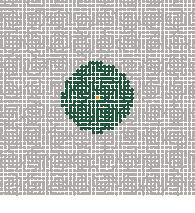
\includegraphics{figures/precompiled/grid_1e-3/points_1.pdf}%
  \quad
  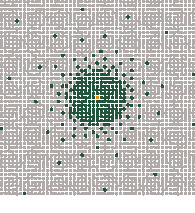
\includegraphics{figures/precompiled/grid_1e-3/points_2.pdf}%
  \quad
  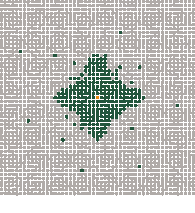
\includegraphics{figures/precompiled/grid_1e-3/points_3.pdf}%
  \quad
  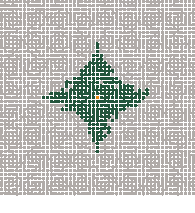
\includegraphics{figures/precompiled/grid_1e-3/points_4.pdf}%
  \caption{
    Dense grid with a random perturbation
    uniformly sampled from \( \pm 10^{-3} \).
  }
\end{figure}

\begin{figure}[H]
  \centering
  % \begin{tikzpicture}[baseline]
  \begin{axis}[
    width={0.25\linewidth},
    height={0.25\linewidth},
    axis lines={none},
    scale only axis=true,
    % legend entries={{}, \( k \)-NN},
    % legend pos={north east},
    legend style={at={(0.9, 0.9)}, anchor=north east},
  ]
  \addplot [only marks, mark size=0.6, silver]   table
    {figures/kernel/grid_1e-2/points.csv};
  \addplot [only marks, mark size=0.6, seagreen] table
    {figures/kernel/grid_1e-2/selected_1.csv};
  \addplot [only marks, mark size=0.6, orange]   table
    {figures/kernel/grid_1e-2/target.csv};
  \end{axis}
\end{tikzpicture}
%
  % \begin{tikzpicture}[baseline]
  \begin{axis}[
    width={0.25\linewidth},
    height={0.25\linewidth},
    axis lines={none},
    scale only axis=true,
    % legend entries={{}, \( \nu = \frac{1}{2} \)},
    % legend pos={north east},
    legend style={at={(0.9, 0.9)}, anchor=north east},
  ]
  \addplot [only marks, mark size=0.6, silver]   table
    {figures/kernel/grid_1e-2/points.csv};
  \addplot [only marks, mark size=0.6, seagreen] table
    {figures/kernel/grid_1e-2/selected_2.csv};
  \addplot [only marks, mark size=0.6, orange]   table
    {figures/kernel/grid_1e-2/target.csv};
  \end{axis}
\end{tikzpicture}
%
  % \begin{tikzpicture}[baseline]
  \begin{axis}[
    width={0.25\linewidth},
    height={0.25\linewidth},
    axis lines={none},
    scale only axis=true,
    % legend entries={{}, \( \nu = \frac{3}{2} \)},
    % legend pos={north east},
    legend style={at={(0.9, 0.9)}, anchor=north east},
  ]
  \addplot [only marks, mark size=0.6, silver]   table
    {figures/kernel/grid_1e-2/points.csv};
  \addplot [only marks, mark size=0.6, seagreen] table
    {figures/kernel/grid_1e-2/selected_3.csv};
  \addplot [only marks, mark size=0.6, orange]   table
    {figures/kernel/grid_1e-2/target.csv};
  \end{axis}
\end{tikzpicture}
%
  % \begin{tikzpicture}[baseline]
  \begin{axis}[
    width={0.25\linewidth},
    height={0.25\linewidth},
    axis lines={none},
    scale only axis=true,
    % legend entries={{}, \( \nu = \frac{5}{2} \)},
    % legend pos={north east},
    legend style={at={(0.9, 0.9)}, anchor=north east},
  ]
  \addplot [only marks, mark size=0.6, silver]   table
    {figures/kernel/grid_1e-2/points.csv};
  \addplot [only marks, mark size=0.6, seagreen] table
    {figures/kernel/grid_1e-2/selected_4.csv};
  \addplot [only marks, mark size=0.6, orange]   table
    {figures/kernel/grid_1e-2/target.csv};
  \end{axis}
\end{tikzpicture}

  \includegraphics{figures/precompiled/grid_1e-2/points_1.pdf}%
  \quad
  \includegraphics{figures/precompiled/grid_1e-2/points_2.pdf}%
  \quad
  \includegraphics{figures/precompiled/grid_1e-2/points_3.pdf}%
  \quad
  \includegraphics{figures/precompiled/grid_1e-2/points_4.pdf}%
  \caption{
    Dense grid with a random perturbation
    uniformly sampled from \( \pm 10^{-2} \).
  }
\end{figure}

\begin{figure}[H]
  \centering
  % \begin{tikzpicture}[baseline]
  \begin{axis}[
    width={0.25\linewidth},
    height={0.25\linewidth},
    axis lines={none},
    scale only axis=true,
    % legend entries={{}, \( k \)-NN},
    % legend pos={north east},
    legend style={at={(0.9, 0.9)}, anchor=north east},
  ]
  \addplot [only marks, mark size=0.6, silver]   table
    {figures/kernel/grid_1e-1/points.csv};
  \addplot [only marks, mark size=0.6, seagreen] table
    {figures/kernel/grid_1e-1/selected_1.csv};
  \addplot [only marks, mark size=0.6, orange]   table
    {figures/kernel/grid_1e-1/target.csv};
  \end{axis}
\end{tikzpicture}
%
  % \begin{tikzpicture}[baseline]
  \begin{axis}[
    width={0.25\linewidth},
    height={0.25\linewidth},
    axis lines={none},
    scale only axis=true,
    % legend entries={{}, \( \nu = \frac{1}{2} \)},
    % legend pos={north east},
    legend style={at={(0.9, 0.9)}, anchor=north east},
  ]
  \addplot [only marks, mark size=0.6, silver]   table
    {figures/kernel/grid_1e-1/points.csv};
  \addplot [only marks, mark size=0.6, seagreen] table
    {figures/kernel/grid_1e-1/selected_2.csv};
  \addplot [only marks, mark size=0.6, orange]   table
    {figures/kernel/grid_1e-1/target.csv};
  \end{axis}
\end{tikzpicture}
%
  % \begin{tikzpicture}[baseline]
  \begin{axis}[
    width={0.25\linewidth},
    height={0.25\linewidth},
    axis lines={none},
    scale only axis=true,
    % legend entries={{}, \( \nu = \frac{3}{2} \)},
    % legend pos={north east},
    legend style={at={(0.9, 0.9)}, anchor=north east},
  ]
  \addplot [only marks, mark size=0.6, silver]   table
    {figures/kernel/grid_1e-1/points.csv};
  \addplot [only marks, mark size=0.6, seagreen] table
    {figures/kernel/grid_1e-1/selected_3.csv};
  \addplot [only marks, mark size=0.6, orange]   table
    {figures/kernel/grid_1e-1/target.csv};
  \end{axis}
\end{tikzpicture}
%
  % \begin{tikzpicture}[baseline]
  \begin{axis}[
    width={0.25\linewidth},
    height={0.25\linewidth},
    axis lines={none},
    scale only axis=true,
    % legend entries={{}, \( \nu = \frac{5}{2} \)},
    % legend pos={north east},
    legend style={at={(0.9, 0.9)}, anchor=north east},
  ]
  \addplot [only marks, mark size=0.6, silver]   table
    {figures/kernel/grid_1e-1/points.csv};
  \addplot [only marks, mark size=0.6, seagreen] table
    {figures/kernel/grid_1e-1/selected_4.csv};
  \addplot [only marks, mark size=0.6, orange]   table
    {figures/kernel/grid_1e-1/target.csv};
  \end{axis}
\end{tikzpicture}

  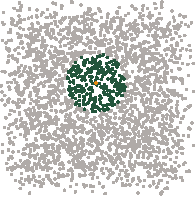
\includegraphics{figures/precompiled/grid_1e-1/points_1.pdf}%
  \quad
  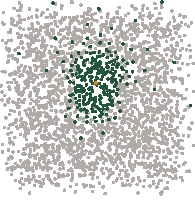
\includegraphics{figures/precompiled/grid_1e-1/points_2.pdf}%
  \quad
  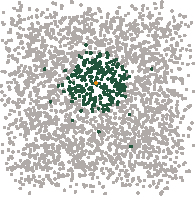
\includegraphics{figures/precompiled/grid_1e-1/points_3.pdf}%
  \quad
  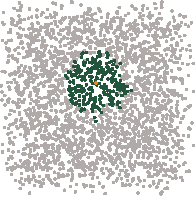
\includegraphics{figures/precompiled/grid_1e-1/points_4.pdf}%
  \caption{
    Dense grid with a random perturbation
    uniformly sampled from \( \pm 10^{-1} \).
  }
\end{figure}

\begin{figure}[H]
  \centering
  % \begin{tikzpicture}[baseline]
  \begin{axis}[
    width={0.25\linewidth},
    height={0.25\linewidth},
    axis lines={none},
    scale only axis=true,
    % legend entries={{}, \( k \)-NN},
    % legend pos={north east},
    legend style={at={(0.9, 0.9)}, anchor=north east},
  ]
  \addplot [only marks, mark size=0.6, silver]   table
    {figures/kernel/maximin_1e-5/points.csv};
  \addplot [only marks, mark size=0.6, seagreen] table
    {figures/kernel/maximin_1e-5/selected_1.csv};
  \addplot [only marks, mark size=0.6, orange]   table
    {figures/kernel/maximin_1e-5/target.csv};
  \end{axis}
\end{tikzpicture}
%
  % \begin{tikzpicture}[baseline]
  \begin{axis}[
    width={0.25\linewidth},
    height={0.25\linewidth},
    axis lines={none},
    scale only axis=true,
    % legend entries={{}, \( \nu = \frac{1}{2} \)},
    % legend pos={north east},
    legend style={at={(0.9, 0.9)}, anchor=north east},
  ]
  \addplot [only marks, mark size=0.6, silver]   table
    {figures/kernel/maximin_1e-5/points.csv};
  \addplot [only marks, mark size=0.6, seagreen] table
    {figures/kernel/maximin_1e-5/selected_2.csv};
  \addplot [only marks, mark size=0.6, orange]   table
    {figures/kernel/maximin_1e-5/target.csv};
  \end{axis}
\end{tikzpicture}
%
  % \begin{tikzpicture}[baseline]
  \begin{axis}[
    width={0.25\linewidth},
    height={0.25\linewidth},
    axis lines={none},
    scale only axis=true,
    % legend entries={{}, \( \nu = \frac{3}{2} \)},
    % legend pos={north east},
    legend style={at={(0.9, 0.9)}, anchor=north east},
  ]
  \addplot [only marks, mark size=0.6, silver]   table
    {figures/kernel/maximin_1e-5/points.csv};
  \addplot [only marks, mark size=0.6, seagreen] table
    {figures/kernel/maximin_1e-5/selected_3.csv};
  \addplot [only marks, mark size=0.6, orange]   table
    {figures/kernel/maximin_1e-5/target.csv};
  \end{axis}
\end{tikzpicture}
%
  % \begin{tikzpicture}[baseline]
  \begin{axis}[
    width={0.25\linewidth},
    height={0.25\linewidth},
    axis lines={none},
    scale only axis=true,
    % legend entries={{}, \( \nu = \frac{5}{2} \)},
    % legend pos={north east},
    legend style={at={(0.9, 0.9)}, anchor=north east},
  ]
  \addplot [only marks, mark size=0.6, silver]   table
    {figures/kernel/maximin_1e-5/points.csv};
  \addplot [only marks, mark size=0.6, seagreen] table
    {figures/kernel/maximin_1e-5/selected_4.csv};
  \addplot [only marks, mark size=0.6, orange]   table
    {figures/kernel/maximin_1e-5/target.csv};
  \end{axis}
\end{tikzpicture}

  \includegraphics{figures/precompiled/maximin_1e-5/points_1.pdf}%
  \quad
  \includegraphics{figures/precompiled/maximin_1e-5/points_2.pdf}%
  \quad
  \includegraphics{figures/precompiled/maximin_1e-5/points_3.pdf}%
  \quad
  \includegraphics{figures/precompiled/maximin_1e-5/points_4.pdf}%
  \caption{
    First points taken from a maximin ordering
    on a perturbed grid at \( \pm 10^{-5} \).
  }
\end{figure}

\begin{figure}[H]
  \centering
  % \begin{tikzpicture}[baseline]
  \begin{axis}[
    width={0.25\linewidth},
    height={0.25\linewidth},
    axis lines={none},
    scale only axis=true,
    % legend entries={{}, \( k \)-NN},
    % legend pos={north east},
    legend style={at={(0.9, 0.9)}, anchor=north east},
  ]
  \addplot [only marks, mark size=0.6, silver]   table
    {figures/kernel/sphere_1e-3/points.csv};
  \addplot [only marks, mark size=0.6, seagreen] table
    {figures/kernel/sphere_1e-3/selected_1.csv};
  \addplot [only marks, mark size=0.6, orange]   table
    {figures/kernel/sphere_1e-3/target.csv};
  \end{axis}
\end{tikzpicture}
%
  % \begin{tikzpicture}[baseline]
  \begin{axis}[
    width={0.25\linewidth},
    height={0.25\linewidth},
    axis lines={none},
    scale only axis=true,
    % legend entries={{}, \( \nu = \frac{1}{2} \)},
    % legend pos={north east},
    legend style={at={(0.9, 0.9)}, anchor=north east},
  ]
  \addplot [only marks, mark size=0.6, silver]   table
    {figures/kernel/sphere_1e-3/points.csv};
  \addplot [only marks, mark size=0.6, seagreen] table
    {figures/kernel/sphere_1e-3/selected_2.csv};
  \addplot [only marks, mark size=0.6, orange]   table
    {figures/kernel/sphere_1e-3/target.csv};
  \end{axis}
\end{tikzpicture}
%
  % \begin{tikzpicture}[baseline]
  \begin{axis}[
    width={0.25\linewidth},
    height={0.25\linewidth},
    axis lines={none},
    scale only axis=true,
    % legend entries={{}, \( \nu = \frac{3}{2} \)},
    % legend pos={north east},
    legend style={at={(0.9, 0.9)}, anchor=north east},
  ]
  \addplot [only marks, mark size=0.6, silver]   table
    {figures/kernel/sphere_1e-3/points.csv};
  \addplot [only marks, mark size=0.6, seagreen] table
    {figures/kernel/sphere_1e-3/selected_3.csv};
  \addplot [only marks, mark size=0.6, orange]   table
    {figures/kernel/sphere_1e-3/target.csv};
  \end{axis}
\end{tikzpicture}
%
  % \begin{tikzpicture}[baseline]
  \begin{axis}[
    width={0.25\linewidth},
    height={0.25\linewidth},
    axis lines={none},
    scale only axis=true,
    % legend entries={{}, \( \nu = \frac{5}{2} \)},
    % legend pos={north east},
    legend style={at={(0.9, 0.9)}, anchor=north east},
  ]
  \addplot [only marks, mark size=0.6, silver]   table
    {figures/kernel/sphere_1e-3/points.csv};
  \addplot [only marks, mark size=0.6, seagreen] table
    {figures/kernel/sphere_1e-3/selected_4.csv};
  \addplot [only marks, mark size=0.6, orange]   table
    {figures/kernel/sphere_1e-3/target.csv};
  \end{axis}
\end{tikzpicture}

  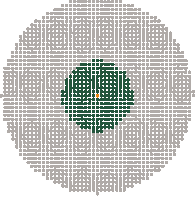
\includegraphics{figures/precompiled/sphere_1e-3/points_1.pdf}%
  \quad
  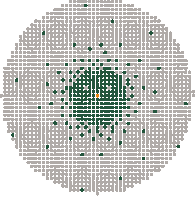
\includegraphics{figures/precompiled/sphere_1e-3/points_2.pdf}%
  \quad
  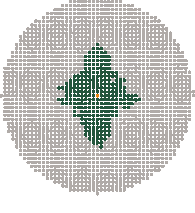
\includegraphics{figures/precompiled/sphere_1e-3/points_3.pdf}%
  \quad
  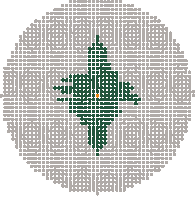
\includegraphics{figures/precompiled/sphere_1e-3/points_4.pdf}%
  \caption{
    Points taken from a regular grid intersected
    with a circular domain and noise \( 10^{-3} \).
  }
\end{figure}

\begin{figure}[H]
  \centering
  % \begin{tikzpicture}[baseline]
  \begin{axis}[
    width={0.25\linewidth},
    height={0.25\linewidth},
    axis lines={none},
    scale only axis=true,
    % legend entries={{}, \( k \)-NN},
    % legend pos={north east},
    legend style={at={(0.9, 0.9)}, anchor=north east},
  ]
  \addplot [only marks, mark size=0.6, silver]   table
    {figures/kernel/sphere_1e-2/points.csv};
  \addplot [only marks, mark size=0.6, seagreen] table
    {figures/kernel/sphere_1e-2/selected_1.csv};
  \addplot [only marks, mark size=0.6, orange]   table
    {figures/kernel/sphere_1e-2/target.csv};
  \end{axis}
\end{tikzpicture}
%
  % \begin{tikzpicture}[baseline]
  \begin{axis}[
    width={0.25\linewidth},
    height={0.25\linewidth},
    axis lines={none},
    scale only axis=true,
    % legend entries={{}, \( \nu = \frac{1}{2} \)},
    % legend pos={north east},
    legend style={at={(0.9, 0.9)}, anchor=north east},
  ]
  \addplot [only marks, mark size=0.6, silver]   table
    {figures/kernel/sphere_1e-2/points.csv};
  \addplot [only marks, mark size=0.6, seagreen] table
    {figures/kernel/sphere_1e-2/selected_2.csv};
  \addplot [only marks, mark size=0.6, orange]   table
    {figures/kernel/sphere_1e-2/target.csv};
  \end{axis}
\end{tikzpicture}
%
  % \begin{tikzpicture}[baseline]
  \begin{axis}[
    width={0.25\linewidth},
    height={0.25\linewidth},
    axis lines={none},
    scale only axis=true,
    % legend entries={{}, \( \nu = \frac{3}{2} \)},
    % legend pos={north east},
    legend style={at={(0.9, 0.9)}, anchor=north east},
  ]
  \addplot [only marks, mark size=0.6, silver]   table
    {figures/kernel/sphere_1e-2/points.csv};
  \addplot [only marks, mark size=0.6, seagreen] table
    {figures/kernel/sphere_1e-2/selected_3.csv};
  \addplot [only marks, mark size=0.6, orange]   table
    {figures/kernel/sphere_1e-2/target.csv};
  \end{axis}
\end{tikzpicture}
%
  % \begin{tikzpicture}[baseline]
  \begin{axis}[
    width={0.25\linewidth},
    height={0.25\linewidth},
    axis lines={none},
    scale only axis=true,
    % legend entries={{}, \( \nu = \frac{5}{2} \)},
    % legend pos={north east},
    legend style={at={(0.9, 0.9)}, anchor=north east},
  ]
  \addplot [only marks, mark size=0.6, silver]   table
    {figures/kernel/sphere_1e-2/points.csv};
  \addplot [only marks, mark size=0.6, seagreen] table
    {figures/kernel/sphere_1e-2/selected_4.csv};
  \addplot [only marks, mark size=0.6, orange]   table
    {figures/kernel/sphere_1e-2/target.csv};
  \end{axis}
\end{tikzpicture}

  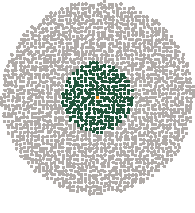
\includegraphics{figures/precompiled/sphere_1e-2/points_1.pdf}%
  \quad
  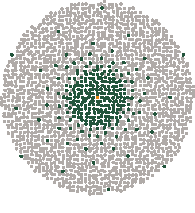
\includegraphics{figures/precompiled/sphere_1e-2/points_2.pdf}%
  \quad
  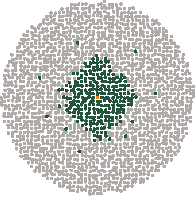
\includegraphics{figures/precompiled/sphere_1e-2/points_3.pdf}%
  \quad
  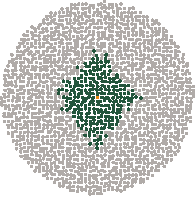
\includegraphics{figures/precompiled/sphere_1e-2/points_4.pdf}%
  \caption{
    Points taken from a regular grid intersected
    with a circular domain and noise \( 10^{-2} \).
  }
\end{figure}

\begin{figure}[H]
  \centering
  % \begin{tikzpicture}[baseline]
  \begin{axis}[
    width={0.25\linewidth},
    height={0.25\linewidth},
    axis lines={none},
    scale only axis=true,
    axis equal image,
    % legend entries={{}, \( k \)-NN},
    % legend pos={north east},
    legend style={at={(0.9, 0.9)}, anchor=north east},
  ]
  \addplot [only marks, mark size=0.6, silver]   table
    {figures/kernel/sarcos1/points.csv};
  \addplot [only marks, mark size=0.6, seagreen] table
    {figures/kernel/sarcos1/selected_1.csv};
  \addplot [only marks, mark size=0.6, orange]   table
    {figures/kernel/sarcos1/target.csv};
  \end{axis}
\end{tikzpicture}
%
  % \begin{tikzpicture}[baseline]
  \begin{axis}[
    width={0.25\linewidth},
    height={0.25\linewidth},
    axis lines={none},
    scale only axis=true,
    axis equal image,
    % legend entries={{}, \( \nu = \frac{1}{2} \)},
    % legend pos={north east},
    legend style={at={(0.9, 0.9)}, anchor=north east},
  ]
  \addplot [only marks, mark size=0.6, silver]   table
    {figures/kernel/sarcos1/points.csv};
  \addplot [only marks, mark size=0.6, seagreen] table
    {figures/kernel/sarcos1/selected_2.csv};
  \addplot [only marks, mark size=0.6, orange]   table
    {figures/kernel/sarcos1/target.csv};
  \end{axis}
\end{tikzpicture}
%
  % \begin{tikzpicture}[baseline]
  \begin{axis}[
    width={0.25\linewidth},
    height={0.25\linewidth},
    axis lines={none},
    scale only axis=true,
    axis equal image,
    % legend entries={{}, \( \nu = \frac{3}{2} \)},
    % legend pos={north east},
    legend style={at={(0.9, 0.9)}, anchor=north east},
  ]
  \addplot [only marks, mark size=0.6, silver]   table
    {figures/kernel/sarcos1/points.csv};
  \addplot [only marks, mark size=0.6, seagreen] table
    {figures/kernel/sarcos1/selected_3.csv};
  \addplot [only marks, mark size=0.6, orange]   table
    {figures/kernel/sarcos1/target.csv};
  \end{axis}
\end{tikzpicture}
%
  % \begin{tikzpicture}[baseline]
  \begin{axis}[
    width={0.25\linewidth},
    height={0.25\linewidth},
    axis lines={none},
    scale only axis=true,
    axis equal image,
    % legend entries={{}, \( \nu = \frac{5}{2} \)},
    % legend pos={north east},
    legend style={at={(0.9, 0.9)}, anchor=north east},
  ]
  \addplot [only marks, mark size=0.6, silver]   table
    {figures/kernel/sarcos1/points.csv};
  \addplot [only marks, mark size=0.6, seagreen] table
    {figures/kernel/sarcos1/selected_4.csv};
  \addplot [only marks, mark size=0.6, orange]   table
    {figures/kernel/sarcos1/target.csv};
  \end{axis}
\end{tikzpicture}

  
\includegraphics{figures/precompiled/sarcos1/points_1.pdf}%
  \quad
  
\includegraphics{figures/precompiled/sarcos1/points_2.pdf}%
  \quad
  
\includegraphics{figures/precompiled/sarcos1/points_3.pdf}%
  \quad
  
\includegraphics{figures/precompiled/sarcos1/points_4.pdf}%
  \caption{
    Points taken from the SARCOS dataset used in \cref{subsec:gp_exp}.
    Note that conditional selection aborts early if the decrease in
    variance is sufficiently small, so there may not be the same number
    of points selected between the panels. In particular, the highest
    smoothness (rightmost) panel selects fewer points.
  }
\end{figure}

\begin{figure}[H]
  \centering
  % \begin{tikzpicture}[baseline]
  \begin{axis}[
    width={0.25\linewidth},
    height={0.25\linewidth},
    axis lines={none},
    scale only axis=true,
    axis equal image,
    % legend entries={{}, \( k \)-NN},
    % legend pos={north east},
    legend style={at={(0.9, 0.9)}, anchor=north east},
  ]
  \addplot [only marks, mark size=0.6, silver]   table
    {figures/kernel/sarcos2/points.csv};
  \addplot [only marks, mark size=0.6, seagreen] table
    {figures/kernel/sarcos2/selected_1.csv};
  \addplot [only marks, mark size=0.6, orange]   table
    {figures/kernel/sarcos2/target.csv};
  \end{axis}
\end{tikzpicture}
%
  % \begin{tikzpicture}[baseline]
  \begin{axis}[
    width={0.25\linewidth},
    height={0.25\linewidth},
    axis lines={none},
    scale only axis=true,
    axis equal image,
    % legend entries={{}, \( \nu = \frac{1}{2} \)},
    % legend pos={north east},
    legend style={at={(0.9, 0.9)}, anchor=north east},
  ]
  \addplot [only marks, mark size=0.6, silver]   table
    {figures/kernel/sarcos2/points.csv};
  \addplot [only marks, mark size=0.6, seagreen] table
    {figures/kernel/sarcos2/selected_2.csv};
  \addplot [only marks, mark size=0.6, orange]   table
    {figures/kernel/sarcos2/target.csv};
  \end{axis}
\end{tikzpicture}
%
  % \begin{tikzpicture}[baseline]
  \begin{axis}[
    width={0.25\linewidth},
    height={0.25\linewidth},
    axis lines={none},
    scale only axis=true,
    axis equal image,
    % legend entries={{}, \( \nu = \frac{3}{2} \)},
    % legend pos={north east},
    legend style={at={(0.9, 0.9)}, anchor=north east},
  ]
  \addplot [only marks, mark size=0.6, silver]   table
    {figures/kernel/sarcos2/points.csv};
  \addplot [only marks, mark size=0.6, seagreen] table
    {figures/kernel/sarcos2/selected_3.csv};
  \addplot [only marks, mark size=0.6, orange]   table
    {figures/kernel/sarcos2/target.csv};
  \end{axis}
\end{tikzpicture}
%
  % \begin{tikzpicture}[baseline]
  \begin{axis}[
    width={0.25\linewidth},
    height={0.25\linewidth},
    axis lines={none},
    scale only axis=true,
    axis equal image,
    % legend entries={{}, \( \nu = \frac{5}{2} \)},
    % legend pos={north east},
    legend style={at={(0.9, 0.9)}, anchor=north east},
  ]
  \addplot [only marks, mark size=0.6, silver]   table
    {figures/kernel/sarcos2/points.csv};
  \addplot [only marks, mark size=0.6, seagreen] table
    {figures/kernel/sarcos2/selected_4.csv};
  \addplot [only marks, mark size=0.6, orange]   table
    {figures/kernel/sarcos2/target.csv};
  \end{axis}
\end{tikzpicture}

  
\includegraphics{figures/precompiled/sarcos2/points_1.pdf}%
  \quad
  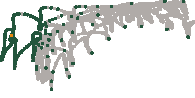
\includegraphics{figures/precompiled/sarcos2/points_2.pdf}%
  \quad
  
\includegraphics{figures/precompiled/sarcos2/points_3.pdf}%
  \quad
  
\includegraphics{figures/precompiled/sarcos2/points_4.pdf}%
  \caption{
    Points taken from the SARCOS dataset.
  }
\end{figure}

\begin{figure}[H]
  \centering
  % \begin{tikzpicture}[baseline]
  \begin{axis}[
    width={0.25\linewidth},
    height={0.25\linewidth},
    axis lines={none},
    scale only axis=true,
    axis equal image,
    % legend entries={{}, \( k \)-NN},
    % legend pos={north east},
    legend style={at={(0.9, 0.9)}, anchor=north east},
  ]
  \addplot [only marks, mark size=0.6, silver]   table
    {figures/kernel/sarcos3/points.csv};
  \addplot [only marks, mark size=0.6, seagreen] table
    {figures/kernel/sarcos3/selected_1.csv};
  \addplot [only marks, mark size=0.6, orange]   table
    {figures/kernel/sarcos3/target.csv};
  \end{axis}
\end{tikzpicture}
%
  % \begin{tikzpicture}[baseline]
  \begin{axis}[
    width={0.25\linewidth},
    height={0.25\linewidth},
    axis lines={none},
    scale only axis=true,
    axis equal image,
    % legend entries={{}, \( \nu = \frac{1}{2} \)},
    % legend pos={north east},
    legend style={at={(0.9, 0.9)}, anchor=north east},
  ]
  \addplot [only marks, mark size=0.6, silver]   table
    {figures/kernel/sarcos3/points.csv};
  \addplot [only marks, mark size=0.6, seagreen] table
    {figures/kernel/sarcos3/selected_2.csv};
  \addplot [only marks, mark size=0.6, orange]   table
    {figures/kernel/sarcos3/target.csv};
  \end{axis}
\end{tikzpicture}
%
  % \begin{tikzpicture}[baseline]
  \begin{axis}[
    width={0.25\linewidth},
    height={0.25\linewidth},
    axis lines={none},
    scale only axis=true,
    axis equal image,
    % legend entries={{}, \( \nu = \frac{3}{2} \)},
    % legend pos={north east},
    legend style={at={(0.9, 0.9)}, anchor=north east},
  ]
  \addplot [only marks, mark size=0.6, silver]   table
    {figures/kernel/sarcos3/points.csv};
  \addplot [only marks, mark size=0.6, seagreen] table
    {figures/kernel/sarcos3/selected_3.csv};
  \addplot [only marks, mark size=0.6, orange]   table
    {figures/kernel/sarcos3/target.csv};
  \end{axis}
\end{tikzpicture}
%
  % \begin{tikzpicture}[baseline]
  \begin{axis}[
    width={0.25\linewidth},
    height={0.25\linewidth},
    axis lines={none},
    scale only axis=true,
    axis equal image,
    % legend entries={{}, \( \nu = \frac{5}{2} \)},
    % legend pos={north east},
    legend style={at={(0.9, 0.9)}, anchor=north east},
  ]
  \addplot [only marks, mark size=0.6, silver]   table
    {figures/kernel/sarcos3/points.csv};
  \addplot [only marks, mark size=0.6, seagreen] table
    {figures/kernel/sarcos3/selected_4.csv};
  \addplot [only marks, mark size=0.6, orange]   table
    {figures/kernel/sarcos3/target.csv};
  \end{axis}
\end{tikzpicture}

  
\includegraphics{figures/precompiled/sarcos3/points_1.pdf}%
  \quad
  
\includegraphics{figures/precompiled/sarcos3/points_2.pdf}%
  \quad
  
\includegraphics{figures/precompiled/sarcos3/points_3.pdf}%
  \quad
  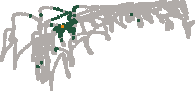
\includegraphics{figures/precompiled/sarcos3/points_4.pdf}%
  \caption{
    Points taken from the SARCOS dataset.
  }
\end{figure}

\bibliographystyle{siamplain}
\bibliography{references}

\end{document}
